% Read the readme first!
% options:
% - uulm-draft: show todonotes, links, linenumbers hide label names
% - uulm-draft-verbose: show todonotes, links, linenumbers, label names
% - uulm-release-electronic: show links, hide todonotes, linenumbers, label names
% - uulm-release-print hide everything
%

\documentclass[uulm-release-electronic]{thesis-uulm} % für die finale Abgabe
%\documentclass[uulm-draft]{thesis-uulm} % um ToDo's anzuzeigen

% workarround for some stupid error in combination with IEEEtran, bibtex and babel.
\makeatletter
\def\markboth#1#2{%
  \def\leftmark{\@IEEEcompsoconly{\sffamily}#1}%
  \def\rightmark{\@IEEEcompsoconly{\sffamily}#2}}
\makeatother

% Choose language
\usepackage[ngerman]{babel}
%% \usepackage[english]{babel}

\usepackage{float}

% Fonts
\renewcommand{\sfdefault}{phv}
\renewcommand{\rmdefault}{phv}
\renewcommand{\ttdefault}{pcr}

% Adjust variables
\author{Lukas Pellot}
\title{Projektionen in D3.js}
\email{lukas.pellot@uni-ulm.de}
\matnr{758179}	% Student ID

\type{Proseminararbeit} % Type of Thesis (Bachelors, Masters)
\jahr{Wintersemester 2017/18}

\gutachterA{Prof. Dr. Timo Ropinski} % First Reviewer
%\gutachterB{Prof. Dr. Un Leserlich}  % Second reviewer
\betreuer{Julian Kreiser} % supervisor

% Can be user to only compile parts of the document
\includeonly{
template/definitions,
chapters/introduction,
chapters/theory,
chapters/projections-in-d3js,
chapters/map-in-d3js,
chapters/choreopleth,
chapters/evaluation,
chapters/content
}

% Definitions for code listings
%% definitions.tex
%%

%Listings für die Darstellung der Treiber im Anhang:
%-------------------------------------------------------
\usepackage{listings}

\usepackage{color}
\definecolor{gray}{rgb}{0.4,0.4,0.4}
\definecolor{darkblue}{rgb}{0.0,0.0,0.6}
\definecolor{cyan}{rgb}{0.0,0.6,0.6}

\lstset{
  basicstyle=\ttfamily,
  columns=fullflexible,
  showstringspaces=false,
  commentstyle=\color{gray}\upshape
}

\lstdefinelanguage{XML}
{
  morestring=[b]",
  morestring=[s]{>}{<},
  morecomment=[s]{<?}{?>},
  stringstyle=\color{black},
  identifierstyle=\color{darkblue},
  keywordstyle=\color{cyan},
  morekeywords={xmlns,version,type}% list your attributes here
}
%-----------------------------------------------------------


\begin{document}

\frontmatter %%%%%%%%%%%%%%%%%%%%%%%%%%%%%%%%%%%%%%%%%%%%%%%%%%%%%%%%%%%%%%%%%
\pagenumbering{roman}
\begin{nolinenumbers}
\maketitle

\copyrightpage % comment out if not wanted
\end{nolinenumbers}

\setstretch{1.2}

\begin{nolinenumbers}
\tableofcontents
\end{nolinenumbers}

\mainmatter %%%%%%%%%%%%%%%%%%%%%%%%%%%%%%%%%%%%%%%%%%%%%%%%%%%%%%%%%%%%%%%%%%
\pagenumbering{arabic}
%% introduction.tex
%%

\chapter{Einleitung}
\label{ch:introduction}

Seit jeher werden Landkarten genutzt, um die topologische Beschaffenheit der Welt sowie, vor allem in Zeiten der Globalisierung, (über-)regionale Sachverhalte und Statistiken grafisch aufbereitet darzustellen.

Allerdings bestehen zwei Problematiken. Dreidimensionale Strukturen wie Globen (und damit auch deren Oberflächen) können aufgrund des "Verlusts" einer Dimension grundsätzlich nur verzerrt auf zweidimensionalen Strukturen (wie Papier oder Computer-Bildschirmen) wiedergegeben werden. Außerdem gibt es unzählige Möglichkeiten, eine solche Verzerrung durchzuführen. Die Vereinheitlichung einer solchen Verzerrung (in Form einer Funktion) nennt man Projektion.

Die vorliegende Ausarbeitung beschäftigt sich mit solchen Projektionen. Es werden zunächst Projektionen im Allgemeinen und danach deren Implementierung und Nutzung in der JavaScript-Bibliothek D3.js erläutert.


%% basics.tex
%%
\chapter{Einführung in Projektionen}
\label{ch:theory}

\section{Allgemeines}

Will man einen Ausschnitt der Oberfläche einer Sphäre, beispielsweise ein Land auf dem Erdball, auf einer ebenen Oberfläche wie einem Bildschirm oder einem Blatt Papier darstellen, so muss eine Funktion aufgestellt werden, die einen dreidimensionalen Punkt (üblicherweise erfolgt die Darstellung hier durch ein Paar aus Breiten- und Längengrad) in einen zweidimensionalen Punkt umwandelt. Eine solche Funktion nennt man Projektion.

Hierbei ist zu beachten, dass mit dem Verlust einer räumlichen Dimension bei der Anwendung einer Projektion stets ein gewisser Informationsverlust beziehungsweise eine -verfälschung einhergeht. Betroffen sein können hierbei der Flächeninhalt der projizierten Struktur, die Länge einer Strecke innerhalb dieser, oder Winkel innerhalb eines Streckenverlaufs. Bewerkstelligt es eine Projektion, bei mehreren projizierten Strukturen eine der genannten Eigenschaften für alle Strukturen um einen konstanten Faktor verzerrt (üblicherweise verkleinert) wiederzugeben, wird diese Projektion flächen-/längen-/winkeltreu genannt.

\section{Kategorisierung von Projektionen}

Projektionen können in folgende Kategorien eingeteilt werden:

\paragraph{Azimutalprojektion}

Bei einer Azimutalprojektion wird die Sphäre ohne Zwischenschritte direkt auf eine Ebene projiziert.

\begin{figure}[H]
    \centering
    
    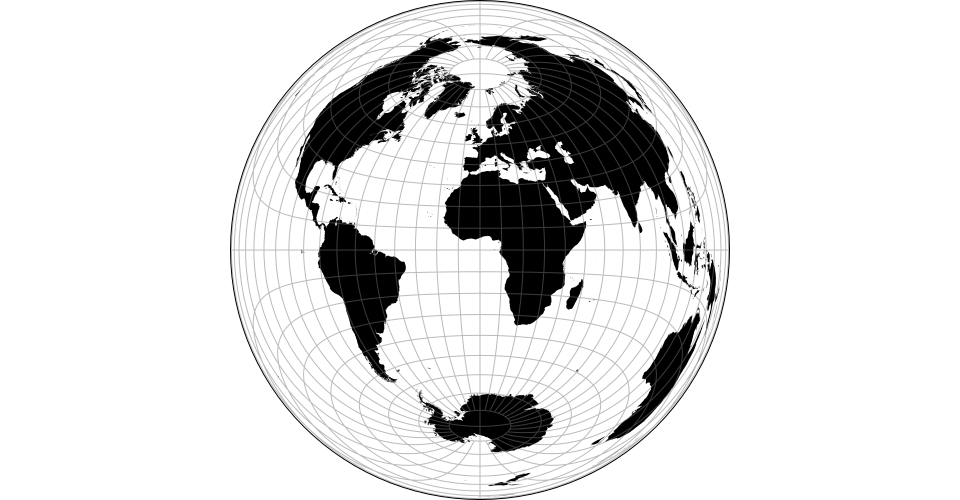
\includegraphics[width=.5\textwidth]{images/azimuthalEqualArea}
    \caption{Flächentreue Azimutalprojektion}
\end{figure}

\begin{figure}[H]
    \centering
    
    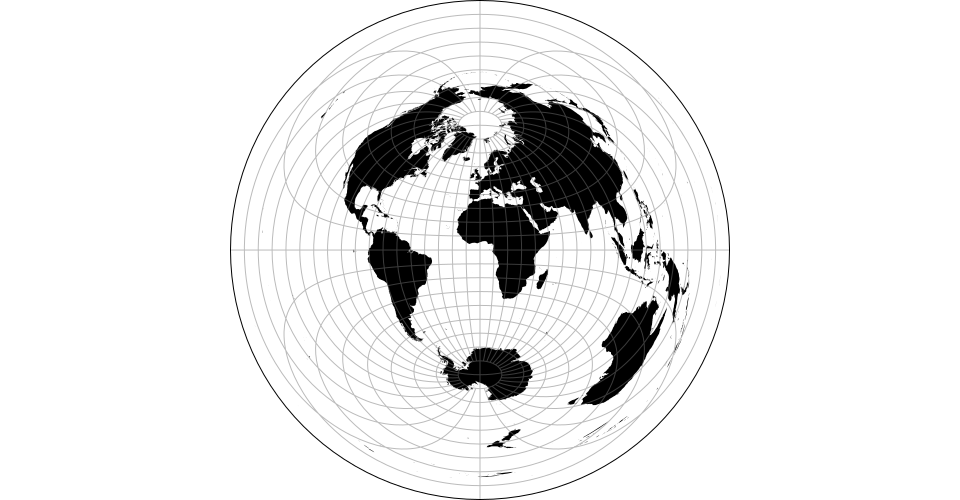
\includegraphics[width=.5\textwidth]{images/azimuthalEquidistant}
    \caption{Längentreue Azimutalprojektion}
\end{figure}

\paragraph{Konische Projektion}

Bei einer konischen Projektion wird die Sphäre zunächst auf einen Kegel projiziert. Dieser wird dann aufgeschnitten und auf eine Ebene ausgerollt.

\begin{figure}[H]
    \centering
    
    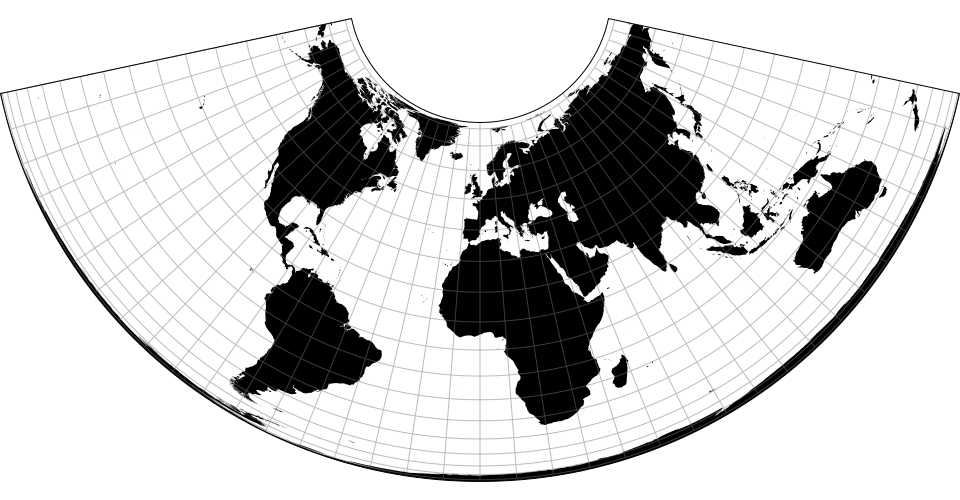
\includegraphics[width=.5\textwidth]{images/conicEqualArea}
    \caption{Flächentreue konische Projektion}
\end{figure}

\begin{figure}[H]
    \centering
    
    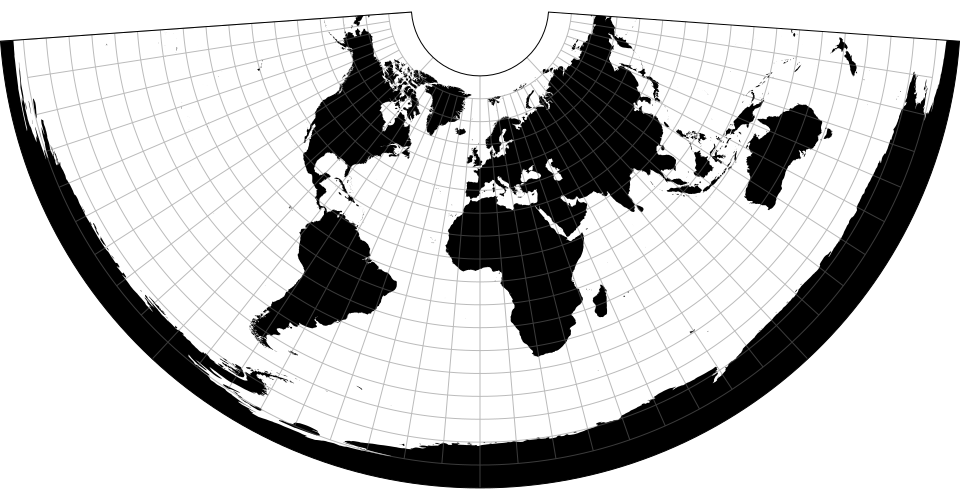
\includegraphics[width=.5\textwidth]{images/conicEquidistant}
    \caption{Längentreue konische Projektion}
\end{figure}

\paragraph{Zylindrische Projektion}

Bei einer zylindrischen Projektion wird die Sphäre zunächst auf einen Zylinder projiziert. Dieser wird dann aufgeschnitten und auf eine Ebene ausgerollt.

\begin{figure}[H]
    \centering
    
    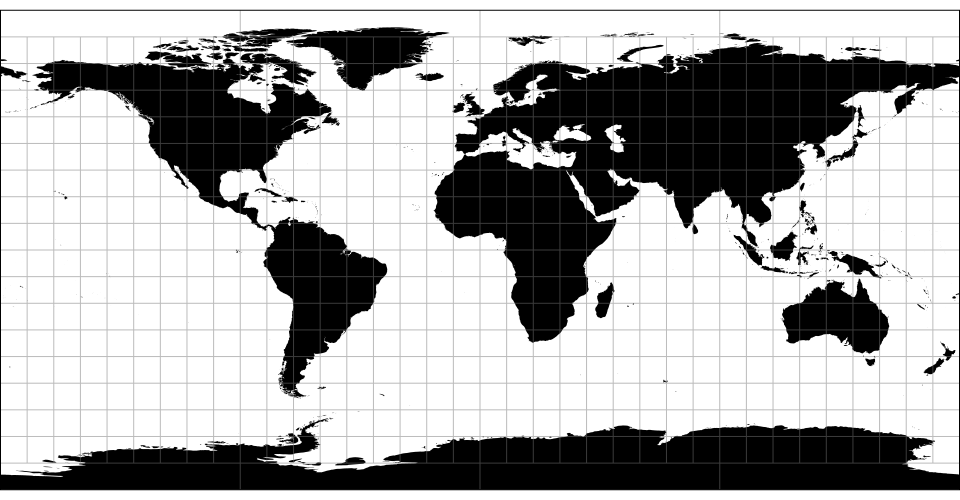
\includegraphics[width=.5\textwidth]{images/equirectangular}
    \caption{Längentreue Zylinderprojektion}
\end{figure}

\begin{figure}[H]
    \centering
    
    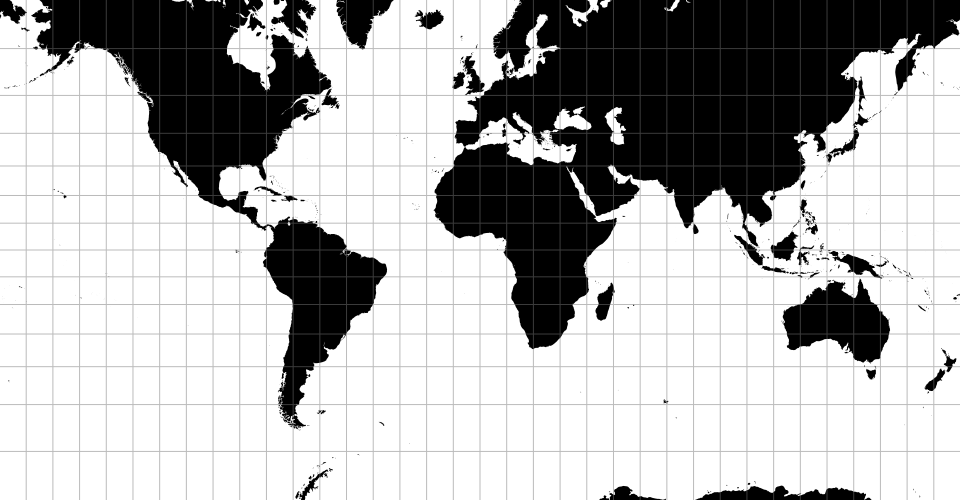
\includegraphics[width=.5\textwidth]{images/mercator}
    \caption{Winkeltreue Zylinderprojektion}
\end{figure}

\paragraph{Pseudozylindrische Projektion}

Pseudozylindrische Projektionen stellen eine Verallgemeinerung zylindrischer Projektionen dar. Breitengrade werden ebenso als parallele Linien projiziert, allerdings sind Höhengrade der konkreten Projektion entsprechend geneigt.

\begin{figure}[H]
    \centering
    
    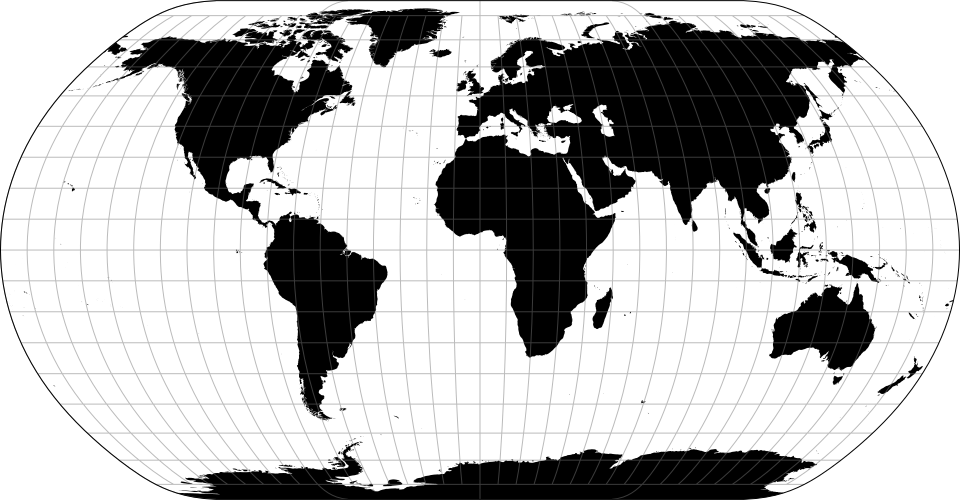
\includegraphics[width=.5\textwidth]{images/naturalEarth1}
    \caption{\glqq Natural Earth\grqq -Projektion}
\end{figure}

\paragraph{Zusammengesetzte Projektion}

Zusammengesetzte Projektionen kombinieren verschiedene der oben genannten Projektionen. Im Gegensatz zu den anderen Kategorien werden zusammengesetzte Projektionen selten für die Darstellung der gesamten Welt, sondern häufiger lediglich für Ausschnitte ebendieser genutzt.

\begin{figure}[H]
    \centering
    
    \includegraphics[width=.5\textwidth]{images/albersUSA}
    \caption{Albers-USA-Projektion}
\end{figure}

Hier wird die Albers-USA-Projektion gezeigt, die den Hauptteil der USA als konische Projektion, allerdings aus Platzgründen Alaska und Hawaii in der linken unteren Ecke um einen Faktor von etwa $0.35$ verkleinert als zylindrische Projektion darstellt.

\paragraph{Anmerkung}

Bei Betrachtung der Abbildungen fällt auf, dass keine der Kategorien Treue hinsichtlich einer Eigenschaft bedingt oder fördert, und diese lediglich der Optik dienlich sind.

%% basics.tex
%%
\chapter{Einführung in Projektionen}

\section{Allgemeines}

Will man einen Ausschnitt der Oberfläche einer Sphäre, beispielsweise ein Land auf dem Erdball, auf einer ebenen Oberfläche wie einem Bildschirm oder einem Blatt Papier darstellen, so muss eine Funktion aufgestellt werden, die einen dreidimensionalen Punkt (üblicherweise erfolgt die Darstellung hier durch ein Paar aus Breiten- und Längengrad) in einen zweidimensionalen Punkt umwandelt. Eine solche Funktion nennt man Projektion.

Hierbei ist zu beachten, dass mit dem Verlust einer räumlichen Dimension bei der Anwendung einer Projektion stets ein gewisser Informationsverlust beziehungsweise eine -verfälschung einhergeht. Betroffen sein können hierbei der Flächeninhalt der projizierten Struktur, die Länge einer Strecke innerhalb dieser, oder Winkel innerhalb eines Streckenverlaufs. Bewerkstelligt es eine Projektion, bei mehreren projizierten Strukturen eine der genannten Eigenschaften für alle Strukturen um einen konstanten Faktor verzerrt (üblicherweise verkleinert) wiederzugeben, wird diese Projektion flächen-/längen-/winkeltreu genannt.

\section{Kategorisierung von Projektionen}

Projektionen können in folgende Kategorien eingeteilt werden:

\paragraph{Azimutalprojektion}

Bei einer Azimutalprojektion wird die Sphäre ohne Zwischenschritte direkt auf eine Ebene projiziert.

\begin{figure}[H]
    \centering
    
    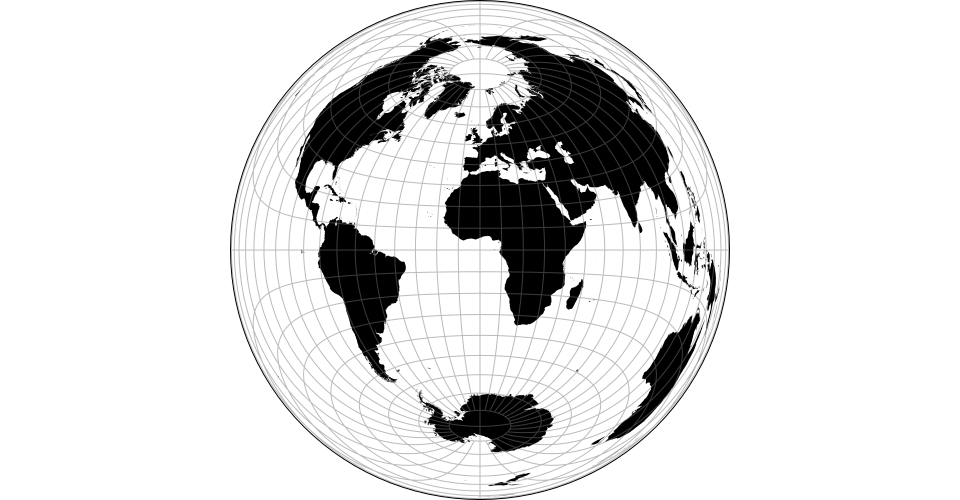
\includegraphics[width=.5\textwidth]{images/azimuthalEqualArea}
    \caption{Flächentreue Azimutalprojektion}
\end{figure}

\begin{figure}[H]
    \centering
    
    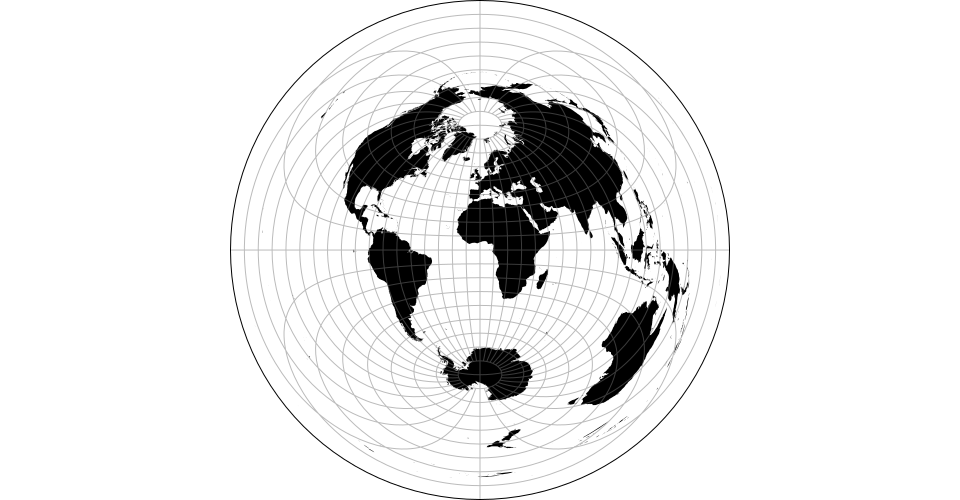
\includegraphics[width=.5\textwidth]{images/azimuthalEquidistant}
    \caption{Längentreue Azimutalprojektion}
\end{figure}

\paragraph{Konische Projektion}

Bei einer konischen Projektion wird die Sphäre zunächst auf einen Kegel projiziert. Dieser wird dann aufgeschnitten und auf eine Ebene ausgerollt.

\begin{figure}[H]
    \centering
    
    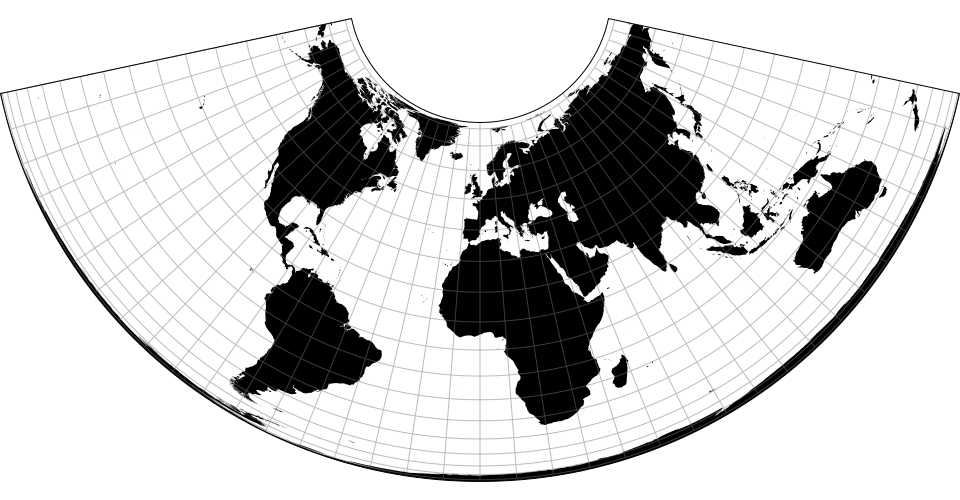
\includegraphics[width=.5\textwidth]{images/conicEqualArea}
    \caption{Flächentreue konische Projektion}
\end{figure}

\begin{figure}[H]
    \centering
    
    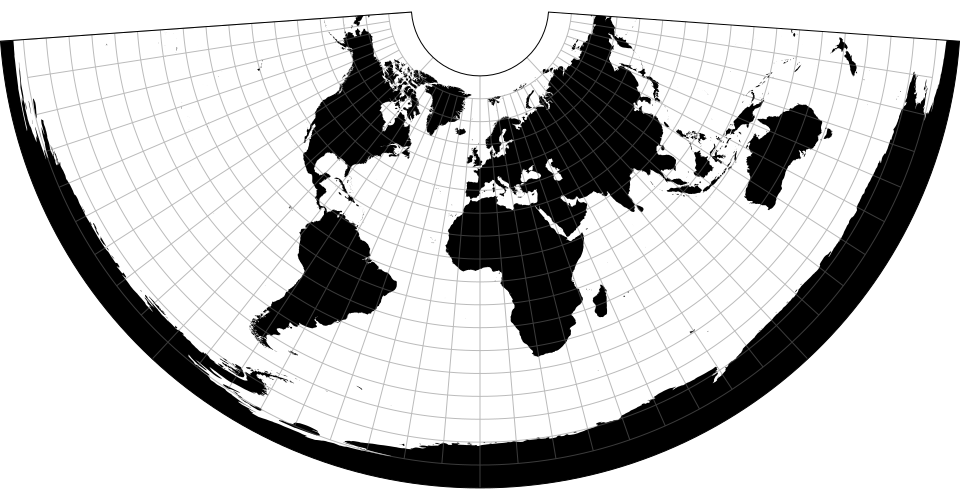
\includegraphics[width=.5\textwidth]{images/conicEquidistant}
    \caption{Längentreue konische Projektion}
\end{figure}

\paragraph{Zylindrische Projektion}

Bei einer zylindrischen Projektion wird die Sphäre zunächst auf einen Zylinder projiziert. Dieser wird dann aufgeschnitten und auf eine Ebene ausgerollt.

\begin{figure}[H]
    \centering
    
    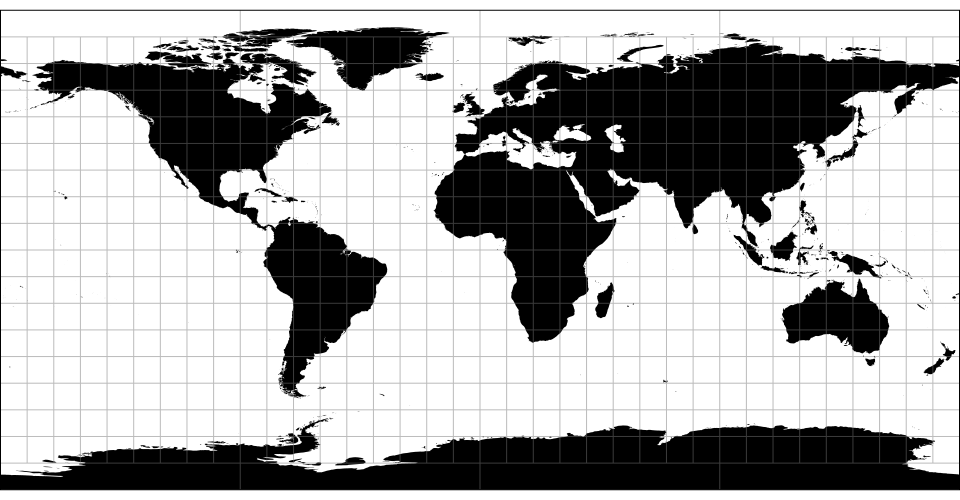
\includegraphics[width=.5\textwidth]{images/equirectangular}
    \caption{Längentreue Zylinderprojektion}
\end{figure}

\begin{figure}[H]
    \centering
    
    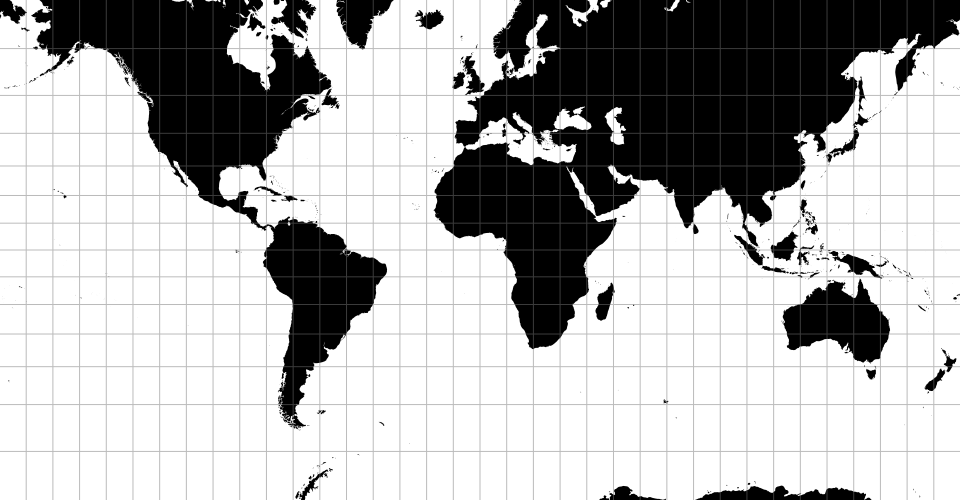
\includegraphics[width=.5\textwidth]{images/mercator}
    \caption{Winkeltreue Zylinderprojektion}
\end{figure}

\paragraph{Pseudozylindrische Projektion}

Pseudozylindrische Projektionen stellen eine Verallgemeinerung zylindrischer Projektionen dar. Breitengrade werden ebenso als parallele Linien projiziert, allerdings sind Höhengrade der konkreten Projektion entsprechend geneigt.

\begin{figure}[H]
    \centering
    
    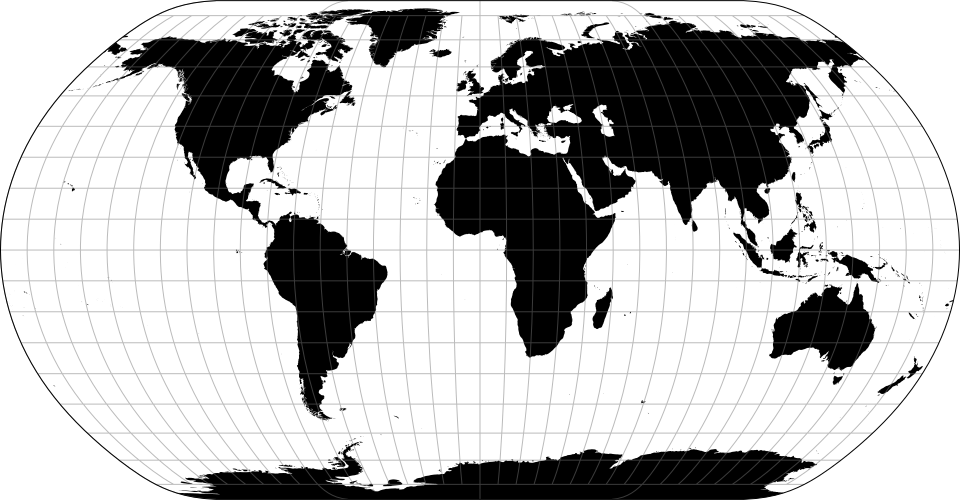
\includegraphics[width=.5\textwidth]{images/naturalEarth1}
    \caption{\glqq Natural Earth\grqq -Projektion}
\end{figure}

\paragraph{Zusammengesetzte Projektion}

Zusammengesetzte Projektionen kombinieren verschiedene der oben genannten Projektionen. Im Gegensatz zu den anderen Kategorien werden zusammengesetzte Projektionen selten für die Darstellung der gesamten Welt, sondern häufiger lediglich für Ausschnitte ebendieser genutzt.

\begin{figure}[H]
    \centering
    
    \includegraphics[width=.5\textwidth]{images/albersUSA}
    \caption{Albers-USA-Projektion}
\end{figure}

Hier wird die Albers-USA-Projektion gezeigt, die den Hauptteil der USA als konische Projektion, allerdings aus Platzgründen Alaska und Hawaii in der linken unteren Ecke um einen Faktor von etwa $0.35$ verkleinert als zylindrische Projektion darstellt.

\paragraph{Anmerkung}

Bei Betrachtung der Abbildungen fällt auf, dass keine der Kategorien Treue hinsichtlich einer Eigenschaft bedingt oder fördert, und diese lediglich der Optik dienlich sind.

%% content.tex
%%
\chapter{Erstellen einer Landkarte in D3.js}
\label{ch:map-in-d3js}

\nocite{blocksmercator:2018}

Im Folgenden wird gezeigt, wie man eine einfache Landkarte in D3.js erstellen kann. Dieser Prozess kann in drei logische Abschnitte aufgeteilt werden.

\section{Allgemeines}
\label{sec:map-abstract}

Zu Beginn müssen ein allgemeine Werte wie Breite und Höhe des Bereichs auf dem Bildschirm sowie ein svg-Tag, in den die Landkarte projiziert werden soll, festgelegt werden.

\begin{lstlisting}

var width = 1440;
var height = 750;

var svg = d3.select("body")
        .append("svg")
        .classed("map", true);

var background = svg.append("rect")
        .attr("width", width)
        .attr("height", height)
        .classed("background", true);

\end{lstlisting}

\section{Anlegen von Projektions- und Pfadfunktion}
\label{sec:map-setup}

Danach müssen die in beschriebenen Projektions- und Pfadfunktionen angelegt werden, mithilfe derer dann die Landkarte gezeichnet werden kann.

\begin{lstlisting}

var projection = d3.geoEquirectangular()
        .scale(width / 2 / Math.PI)
        .translate([width / 2, height / 2]);

var path = d3.geoPath()
        .projection(projection);

\end{lstlisting}

\section{Einlesen und Verarbeiten der zu projizierenden Daten}

Zuletzt muss noch die Datei, welche die zu projizierenden Daten repräsentiert, eingelesen und verarbeitet werden.

\begin{lstlisting}

var url = "..."; // URL, die auf die zu verarbeitende Datei verweist

d3.json(url, function(geojson){
    svg.append("path")
            .attr("d", path(geojson));
});

\end{lstlisting}

Die entstehende Landkarte hat dieses Aussehen:

\begin{figure}[H]
    \centering
    
    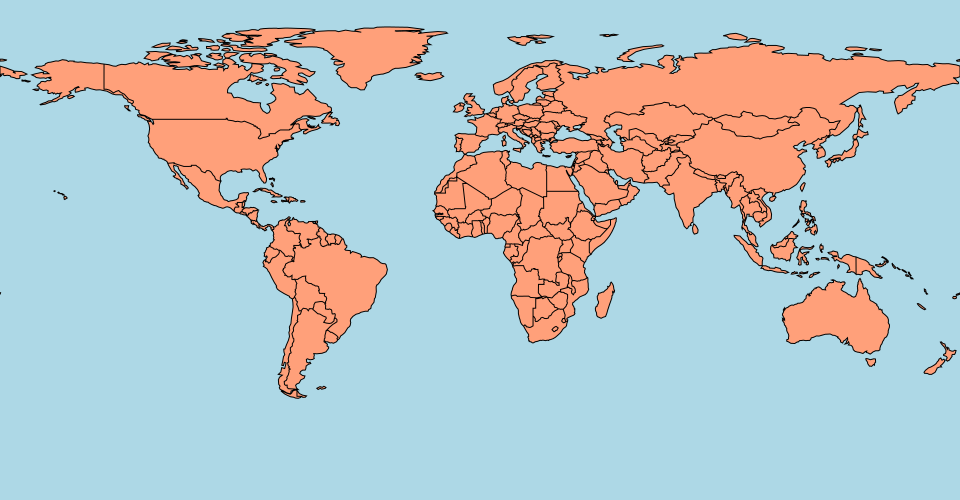
\includegraphics[width=.5\textwidth]{images/mapSinglePath}
    \caption{\glqq Natural Earth\grqq -Projektion}
\end{figure}
%% content.tex
%%
\chapter{Choreoplethen-Karten}
\label{choreopleth}

\nocite{blocksmercator:2018}
\nocite{blockscolombia:2018}

\section{Allgemeines}
\label{sec:choreopleth-abstract}

Choreoplethenkarten unterscheiden sich von gewöhnlichen/einfachen Landkarten darin, dass bestimmte Abschnitte einer Karten einer bestimmten statistischen Variablen entsprechend eingefärbt werden. Daher rührt auch ihre alternative Bezeichnung als 'Thematische Karten'.

Nützlich ist diese Art einer Landkarte vor allem, um zu zeigen, wie Messungen/Werte in bestimmten geographischen Regionen variieren, sowie daraus gegebenenfalls Schlüsse zu ziehen. Ein Beispiel hierfür wäre die Anzahl erwerbsloser Personen in Relation zur Einwohnerzahl für jeden Landkreis in Deutschland.

\section{Implementierung in D3.js}
\label{sec:choreopleth-implementation}

\subsection{Problematik bzgl. bisherigem Ansatz}

Beim Versuch, eine solche Choreoplethenkarten in D3.js zu implementieren, tritt ein Problem mit der bisherigen Implementierung auf. Diese bildet zwar alle Länder ab, nutzt hierzu aber lediglich einen einzelnen Pfad, welcher folglich auch nur mit einer einzelnen Farbe gefüllt werden kann, was die Vergleichbarkeit von Regionen unmöglich macht.

Man muss also zunächst die Implementierung so abändern, dass statt einem Pfad für alle Länder ein Pfad pro Land gezeichnet wird. Möglich wird dies, wenn man statt dem übergebenen GeoJSON-Objekt als Ganzes nur das "features"-Array unter Zuhilfenahme des Enter-Update-Exit-Patterns an die Funktion übergibt.

\subsection{Implementierungsansatz zur Bewältigung}

Der allgemeine Teil und der Teil zum Anlegen von Projektions- und Pfadfunktion gestalten sich wie in \ref{sec:map-abstract} und \ref{sec:map-setup} beschrieben. Danach folgt das veränderte Einlesen der Datei wie folgt:

\begin{lstlisting}

var url = "...";

d3.json(url, function(geojson){
    svg.selectAll("path")
            .data(geojson.features)
            .enter()
            .append("path")
            .attr("d", path);
})

\end{lstlisting}

\subsection{Einfärbung der Landkarte}

Um nun noch gemäß der Aufgabenstellung jedes Land entsprechend seiner Kennzahl einfärben zu können, muss eine Farbskala erstellt werden. Beim Zeichnen der Pfade wird dann die jeweilige Füllfarbe mithilfe des Werts der entsprechenden Kennzahl und der Farbskala berechnet und gesetzt.

Der allgemeine Teil und der Teil zum Anlegen von Projektions- und Pfadfunktion gestalten sich erneut wie in \ref{sec:map-abstract} und \ref{sec:map-setup} beschrieben. Danach folgt das Einlesen der Datei und Einfärben der Pfade wie folgt (Kennzahl ist das Bruttoinlandsprodukt jeden Landes, das in der GeoJSON-Datei über den optionalen Wert "properties" mit übergeben wird)

\begin{lstlisting}

var url = "...";

d3.json(url, function(geojson){
    var features = geojson.features;

    var min = d3.min(features, function(d){
        return d.properties.gdp_md_est;
    });

    var max = d3.max(features, function(d){
        return d.properties.gdp_md_est;
    });

    var color = d3.scaleLinear()
            .domain([min, max])
            .range(["white", "crimson"]);

    svg.selectAll("path")
            .data(features)
            .enter()
            .append("path")
            .attr("d", path)
            .style("fill", function(d){
                return color(d.properties.gdp_md_est);
            });
});

\end{lstlisting}

Die entstehende Landkarte hat dieses Aussehen:

\begin{figure}[H]
    \centering
    
    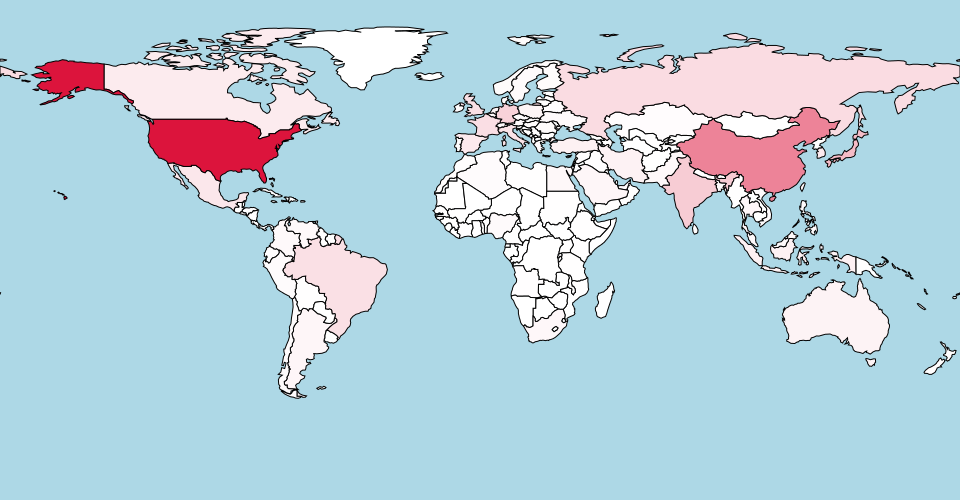
\includegraphics[width=.5\textwidth]{images/mapChoreopleth}
    \caption{\glqq Natural Earth\grqq -Projektion}
\end{figure}
%% evaluation.tex
%%

\chapter{Abschluss}
\label{ch:conclusion}

Wie in dieser Arbeit gezeigt wurde, kann in D3.js ohne großen Aufwand eine Landkarte erstellt und nach Belieben eingefärbt werden. Abschließend gilt zu sagen, dass die Möglichkeit besteht, Landkarten jeder Art in D3.js beliebig zu gestalten, und man keinesfalls auf rein optische Vorgänge beschränkt ist. 

So ist zum Beispiel eine interaktive Gestaltung der Karte innerhalb von D3.js möglich, indem man gezeichneten Pfaden Maus- oder sonstige Ereignisse und deren Verarbeitung zuweist. In entsprechender Fachliteratur wie der offiziellen Dokumentation finden sich viele weitere Ansätze zur Gestaltung.
%% content.tex
%%
\chapter{Illustrationen}
\label{ch:illustrationen}

\section{Bilder}
\label{ch:illustrationen:sec:images}

Bilder kann man natürlich auch in Arbeiten integrieren.
Für Fotos und Ähnliches unterstützt PDF-\LaTeX{} direkt \verb|jpg| und \verb|png|, ansonsten empfiehlt es sich Vektorgrafiken zu verwenden und diese als \verb|pdf| zu speichern.
Sollte ein Bild einmal zu viel weißen Raum um sich haben, so kann man mit dem Werkzeug \verb|pdfcrop| das Bild automatisch ausschneiden\cite{pdfcrop}.

\begin{figure} [ht]
\centering
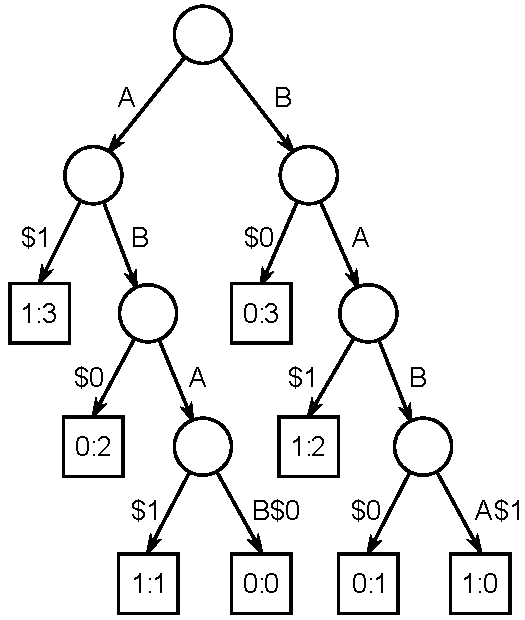
\includegraphics[width=.4\textwidth]{images/Suffix_tree_ABAB_BABA}
\caption{Beschreibung/Beschriftung des Bilds}
\label{fig:bild1}
\end{figure}

Mit Hilfe eines Labels kann man sich dann im Text auf diese Grafik (\ref{fig:bild1}) beziehen. 

\section{Tabellen}
\label{ch:illustrationen:sec:tables}

Seite \pageref{tab:beispieltabelle} enthält Beispieltabelle \ref{tab:beispieltabelle}.
In jedem \LaTeX{}-Buch finden sich gute Anleitungen zum Erstellen von Tabellen.
Komplexere Tabellen können in Excel vorgefertigt und mit Excel2LaTeX, einem Add-in von Excel, nach LaTeX konvertiert werden.

\begin{table}[h]
\begin{center}
\begin{tabular}{|l|l|l|}
	A & B & C \\\hline
	x & x & x \\
	x & x & x
\end{tabular}
\end{center}
\caption{Eine kleine Beispieltabelle}
\label{tab:beispieltabelle}
\end{table}

\section{Formeln}
\label{ch:illustrationen:sec:formula}

sec Formeln lassen sich in der Umgebung  \verb|math| erzeugen.
Die Kurz- Schreibweise lautet \verb|\( a^2+b^2=c^2 \)|;  hierbei steht die Formel dann im laufenden Text: \( a^2+b^2=c^2 \).
Die kürzeste Form ist mit zwei \verb|$| um die Formel, z.B.~so: Wasser ist H$_2$O.

Mit der Schreibweise \verb|\[ y=x^2 \]| wird die Formel mittig in einer eigenen Zeile gesetzt, z.B.

\[y = x^2 \]

Formeln in der Umgebung \verb|equation| werden mittig in einer eigenen Zeile gesetzt und fortlaufend nummeriert:

\begin{equation}
x_{1,2} = \frac{-b\pm\sqrt{b^2-4ac}}{2a}
\label{mitternachtsformel}
\end{equation}
Wenn wir z.B.~über die beliebte Mitternachtsformel (Gleichung \ref{mitternachtsformel}) Details im umliegenden Text schreiben wollen, lässt sich diese wie ein Bild referenzieren.

\section{Quellcode}
\label{ch:illustrationen:sec:code}

Quellcode und ähnlich zu formatierende Texte können mit \verb|verbatim| in einer Umgebung gesetzt werden.

\begin{verbatim}
Dieser Text ist in Schreibmaschinenschrift
\end{verbatim}

Schöner geht es mit dem \verb|listings|-Paket, das Quelltext auch entsprechend formatiert.
Dazu kann man in der Präambel die Sprache angeben, in der die Quellcodes geschrieben sind.

\begin{lstlisting}
public class Hello {
    public static void main(String[] args) {
        System.out.println("Hello World");
    }
}
\end{lstlisting}

Im Text gibt man Wörter am Besten als \verb|\verb##| an, dabei erwartet \LaTeX{} zweimal das gleiche Zeichen als Begrenzer.
Im Beispiel ist dies die Raute \verb|#|, man kann aber ein anderes Zeichen nehmen, z.B. das Plus .

\section{Text}
\label{ch:illustrationen:sec:text}

Text kann mit dem Befehl \verb|\emph{}| \emph{hervorgehoben} werden.
Falls in einem Satz ein Punkt vorkommt, macht man vor ihm kein Leerzeichen sondern eine Tilde (\verb|~|), denn dann fügt \LaTeX{} den korrekten Abstand ein, z.B.~so.

\begin{verbatim}
z.B.~so
\end{verbatim}

In der Präambel der vorliegenden tex-Datei gibt es den Befehl \verb|hypenation|, der zur Silbentrennung da ist.
\LaTeX{} verfügt zwar über  eine eingebaute Silbentrennung, die jedoch bei manchen Wörtern falsch trennt.
Damit diese Wörter korrekt getrennt werden, gibt man sie dann mit dem Befehl in der Präambel an\footnote{Das Wort \emph{Silbentrennung} ist hier das Beispiel}.

Fußnoten werden mit dem Befehl \verb|footnote| mitten in den fortlaufenden Text eingefügt. \footnote{Wie man schon im vorherigen Absatz sehen konnte.}.

In wissenschaftlichen Arbeiten muss man des öfteren andere Arbeiten zitieren.
Dazu nutzt man den Befehl \verb|\cite{name}|.
In eckigen Klammern kann man noch die Seitenzahl angeben, falls notwendig.
Der Name ist ein Schlüssel aus der Datei \verb|bibliography.bib| \cite[S.~10]{kopka}.
Falls einmal ein Werk nur indirekt zu einem Teil der Arbeit beigetragen hat, kann man es auch mit \verb|nocite| angeben, dann landet es in der Literaturliste, ohne dass es im Text ausdrücklich zitert wird.

\subsection{Weiterführendes}

Zum Schluss sei auf die Vielzahl an Büchern zu \LaTeX{} verwiesen.
In jeder Bibliothek wird sich eine Einführung finden, in der dann weitere Themen wie mathematische Formeln, Aufbau von Briefen und viele nützliche Erweiterungen besprochen werden.


\backmatter %%%%%%%%%%%%%%%%%%%%%%%%%%%%%%%%%%%%%%%%%%%%%%%%%%%%%%%%%%%%%%%%%%

%\bibliographystyle{natdin}
\bibliographystyle{IEEEtranS}	% alternativer Stil
\bibliography{bibliography} % Bib-Datei

\end{document}
